\documentclass{article}

\usepackage{amsmath,amsthm,amssymb}
\usepackage{commath}
\usepackage{mathtools}
\usepackage{enumerate}
\usepackage{subcaption}
\usepackage{float}
\usepackage{tikz}
\usepackage[margin=.8in]{geometry}
\usepackage{multicol}
\usepackage{epstopdf}
\usepackage[linesnumbered]{algorithm2e}

\newenvironment{algorithmic}{%
\renewenvironment{algocf}[1][h]{}{}% pass over the floating stuff
\algorithm
}{%
\endalgorithm
}

\usetikzlibrary{positioning, shapes, automata, arrows, backgrounds, shapes.geometric}

\setlength{\parindent}{0pt}
\setlength{\parskip}{8pt}

\usepackage[utf8]{inputenc}
\begin{document}
\title{Assignment 11 \\ Advanced Algorithms \& Data Structures PS}%
\author{Christian Müller 1123410 \\ Daniel Kocher, 0926293}%
\maketitle

{\bfseries Aufgabe 21}%

Gegeben sei folgende Sequenz $I$ von Objekten
\begin{equation}
\frac{1}{16}+\epsilon,...,\frac{1}{16}+\epsilon,\frac{1}{8}+\epsilon,...,\frac{1}{8}+\epsilon,\frac{1}{4}+\epsilon,...,\frac{1}{4}+\epsilon,\frac{1}{2}+\epsilon,...,\frac{1}{2}+\epsilon
\end{equation}
wobei jede Teilsequenz (Objekte der gleichen Größe) die Länge $16m $ hat.\\ Es gilt $m\in N: $ $0 \equiv m \pmod{15}$ $\wedge$ $0 \equiv m \pmod{7}$ $\wedge$ $0 \equiv m \pmod{3}$ und $\epsilon < 10^{-6}$.
\begin{itemize}
	\item Geben Sie $FF(I)$ sowie die zugehörige Packung an.
	\item Wenden Sie First-Fit-Decreasing auf $I$ an. Geben Sie die zugehörige Packung sowie $FFD(I)$ an.
\end{itemize}

\begin{figure}[H]
\begin{center}
	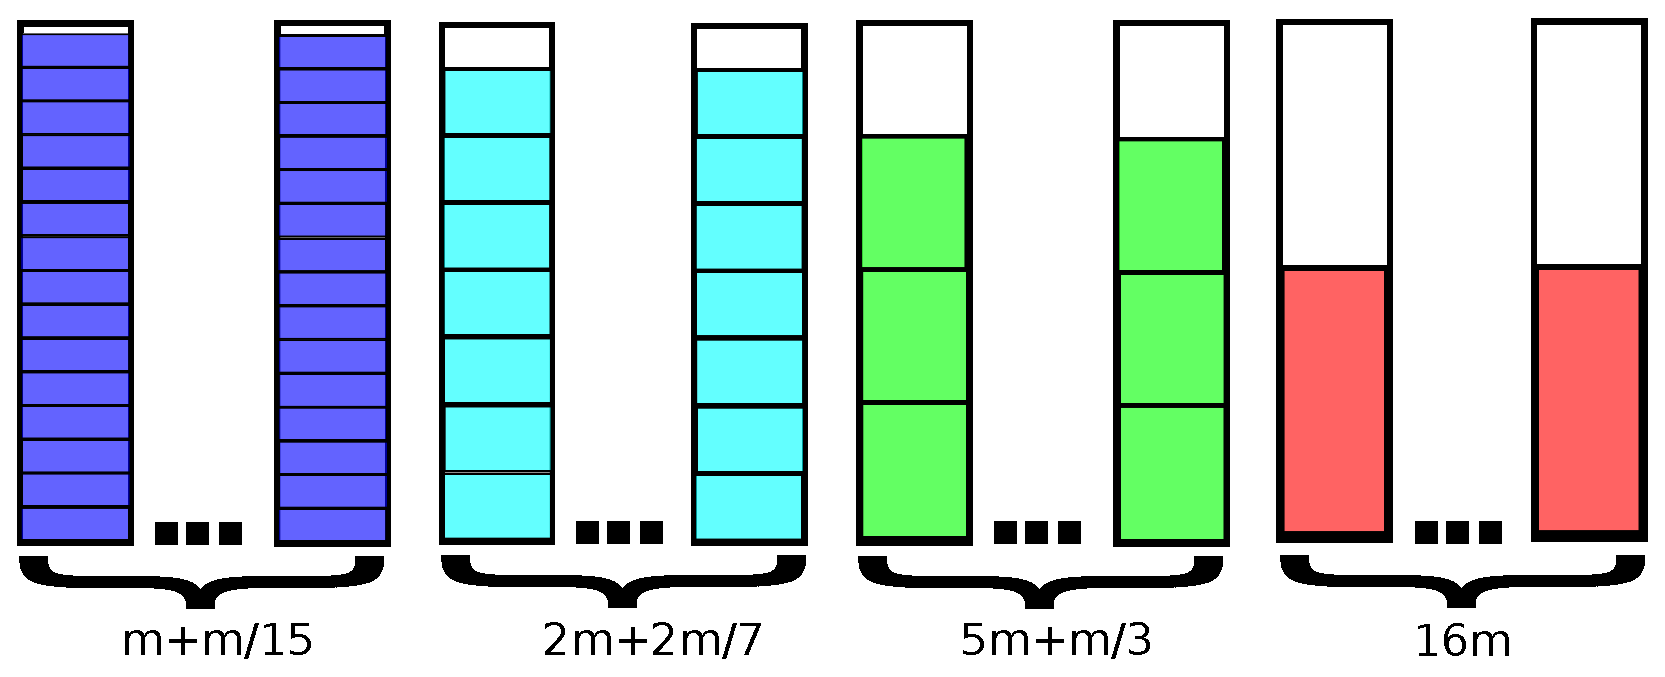
\includegraphics[scale=.5]{drawing}
\end{center}
\end{figure}
Aufteilung der $16m$ Elemente der Größe  $\frac{1}{16}+\epsilon$. \\
Eine Runde sei das Einfügen von $16$ Elementen. Also ist nach $m$ Runden das Einfügen von $16m$ Elementen beendet.\\

Runde 1: $B_{1}: 15\cdot(\frac{1}{16}+\epsilon), B_{2}:(\frac{1}{16}+\epsilon) $\\
Runde 2: $B_{1}: 15\cdot(\frac{1}{16}+\epsilon), B_{2}:15\cdot(\frac{1}{16}+\epsilon), B_{3}: 2\cdot(\frac{1}{16}+\epsilon) $\\
Runde 3: $B_{1}: 15\cdot(\frac{1}{16}+\epsilon), B_{2}:15\cdot(\frac{1}{16}+\epsilon), B_{3}: 15\cdot(\frac{1}{16}+\epsilon),B_{4}: 3\cdot(\frac{1}{16}+\epsilon)  $\\
...\\
Runde 15: $B_{1}: 15\cdot(\frac{1}{16}+\epsilon), B_{2}:15\cdot(\frac{1}{16}+\epsilon), B_{3}: 15\cdot(\frac{1}{16}+\epsilon),B_{4}: 15\cdot(\frac{1}{16}+\epsilon), ...,B_{16}: 15\cdot(\frac{1}{16}+\epsilon) $


wegen $0 \equiv m \pmod{15}$ gilt:\\
Runde m: $B_{1}: 15\cdot(\frac{1}{16}+\epsilon), B_{2}:15\cdot(\frac{1}{16}+\epsilon), B_{3}: 15\cdot(\frac{1}{16}+\epsilon),B_{4}: 15\cdot(\frac{1}{16}+\epsilon), ...,B_{m+\frac{m}{15}}: 15\cdot(\frac{1}{16}+\epsilon) $

Alle $m+\frac{m}{15}$ Blöcke sind nach $m$ Runden vollständig gefüllt.
Nach $m$ Runden gilt für alle Blöcke $B_{j}$ mit $1\leq j \leq m+\frac{m}{15}$ also: 
\begin{equation}
B_{j} + (\frac{1}{16}+\epsilon) > 1
\end{equation}
Aufgrund der gegebenen Einfügereihenfolge  bedeutet das also, dass diesen Blöcken kein weiteres Element der Restsequenz mehr hinzugefügt werden kann, da diese alle eine Größe haben, die $(\frac{1}{16}+\epsilon)$ übersteigt.


Aufteilung der $16m$ Elemente der Größe  $\frac{1}{8}+\epsilon$. \\

\begin{center}
  \begin{tabular}{| l | c | c | c | c | c | c |  }
    \hline
    $B_{k}$ & Runde 1 & Runde 2 & ... & Runde 7 & ... & Runde m\\ \hline
    $(m+\frac{m}{15})+1$ & $7\cdot(\frac{1}{8}+\epsilon)$ & $7\cdot(\frac{1}{8}+\epsilon)$ & $...$ & $7\cdot(\frac{1}{8}+\epsilon)$ & $...$ & $7\cdot(\frac{1}{8}+\epsilon)$ \\ \hline
    $(m+\frac{m}{15})+2$ & $7\cdot(\frac{1}{8}+\epsilon)$ & $7\cdot(\frac{1}{8}+\epsilon)$ & $...$ & $7\cdot(\frac{1}{8}+\epsilon)$ & $...$ & $7\cdot(\frac{1}{8}+\epsilon)$  \\ \hline
    $(m+\frac{m}{15})+3$ & $2\cdot(\frac{1}{8}+\epsilon)$ & $7\cdot(\frac{1}{8}+\epsilon)$ & $...$ & $7\cdot(\frac{1}{8}+\epsilon)$ & $...$ & $7\cdot(\frac{1}{8}+\epsilon)$  \\ \hline
    $(m+\frac{m}{15})+4$ & $/$ & $7\cdot(\frac{1}{8}+\epsilon)$ & $...$ & $7\cdot(\frac{1}{8}+\epsilon)$ & $...$ & $7\cdot(\frac{1}{8}+\epsilon)$  \\ \hline
    $(m+\frac{m}{15})+5$ & $/$ & $4\cdot(\frac{1}{8}+\epsilon)$ & $...$ & $7\cdot(\frac{1}{8}+\epsilon)$ & $...$ & $7\cdot(\frac{1}{8}+\epsilon)$  \\ \hline
 	$(m+\frac{m}{15})+6$ & $/$ & $/$ & $...$ & $7\cdot(\frac{1}{8}+\epsilon)$ & $...$ & $7\cdot(\frac{1}{8}+\epsilon)$  \\ \hline
    $...$  & $...$ & $...$ & $...$ & $...$ & $...$ & $...$  \\ \hline
    $(m+\frac{m}{15})+16$ & $/$ & $/$ & $...$ & $7\cdot(\frac{1}{8}+\epsilon)$ & $...$ & $7\cdot(\frac{1}{8}+\epsilon)$ \\ \hline
      $(m+\frac{m}{15})+17$ & $/$ & $/$ & $...$ & $/$ & $...$ & $7\cdot(\frac{1}{8}+\epsilon)$ \\ \hline
    $...$ & $...$ & $...$ & $...$ & $...$ & $...$ & $...$  \\ \hline
    $(m+\frac{m}{15})+(2m+\frac{2m}{7})$ & $/$ & $/$ & $...$ & $/$ & $...$ & $7\cdot(\frac{1}{8}+\epsilon)$  \\ \hline
    \hline
  \end{tabular}
\end{center}

$16$ Objekte der Größe ($\frac{1}{8}+\epsilon$) füllen (d.h. sodass kein weiteres Objekt dieser Größe Platz hat)  $2$ Blöcke und es bleiben $2$ Objekte übrig. Im Rahmen von $k$ Runden wächst dieser Rest auf $2k$ Objekte an. Um diese $2k$ zusätzlichen Objekte unterzubringen, werden $\lceil\frac{2k}{7}\rceil$ zusätzliche Blöcke benötigt.

Analog für $\frac{1}{4}+\epsilon$ und $\frac{1}{2}+\epsilon$

\begin{align*}
FF(I)=m+\frac{m}{15}+2m+\frac{2m}{7}+5m+\frac{m}{3}+16m\\
=24m+\frac{m}{15}+\frac{2m}{7}+\frac{m}{3}\\
=24m+\frac{7m+30m+35m}{105}\\
=24m+\frac{24m}{35}
\end{align*}
Für das Einfügen der Sequenz $I$ ($64m$ Elemente) werden $24m+\lceil\frac{24m}{35}\rceil$ Container benötigt.
\newpage
Wenden Sie First-Fit-Decreasing auf $I$ an. Geben Sie die zugehörige Packung sowie $FFD(I)$ an.\\
Sortiere Sequenz $I$, sodass die Elemente in absteigender Reihenfolge vorliegen:\\
\begin{equation}
\frac{1}{2}+\epsilon,...,\frac{1}{2}+\epsilon,\frac{1}{4}+\epsilon,...,\frac{1}{4}+\epsilon,\frac{1}{8}+\epsilon,...,\frac{1}{8}+\epsilon,\frac{1}{16}+\epsilon,...,\frac{1}{16}+\epsilon
\end{equation}
wobei jede Teilsequenz (Objekte der gleichen Größe) die Länge $16m $ hat.\\ Es gilt $m\in N: $ $0 \equiv m \pmod{15}$ $\wedge$ $0 \equiv m \pmod{7}$ $\wedge$ $0 \equiv m \pmod{3}$ und $\epsilon < 10^{-6}$.
\begin{multicols}{2}
Nach Einfügen der $16m$ $\frac{1}{2}+\epsilon$ Objekte. 
\begin{figure}[H]
\begin{center}
	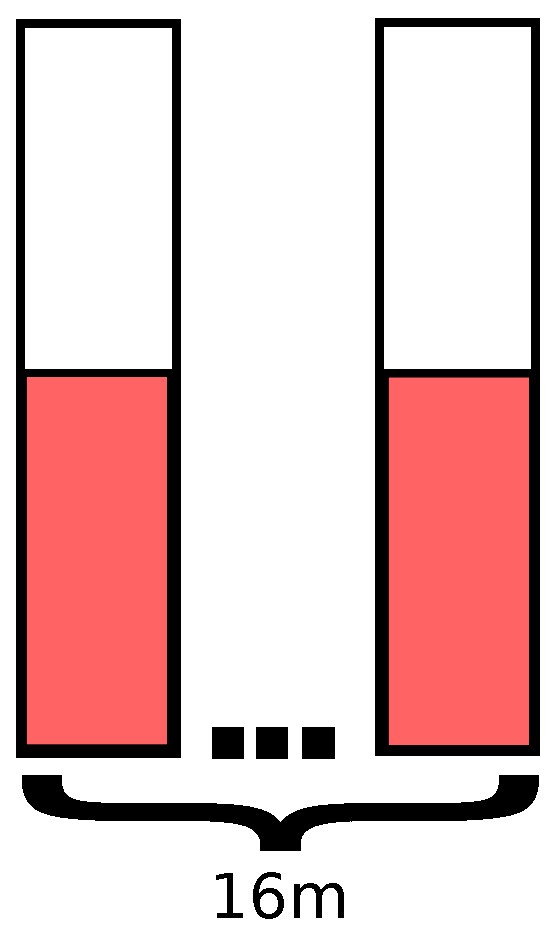
\includegraphics[scale=.3]{first}
\end{center}
\end{figure}
\columnbreak%
Nach Einfügen der $16m$ $\frac{1}{4}+\epsilon$ Objekte. 
\begin{figure}[H]
\begin{center}
	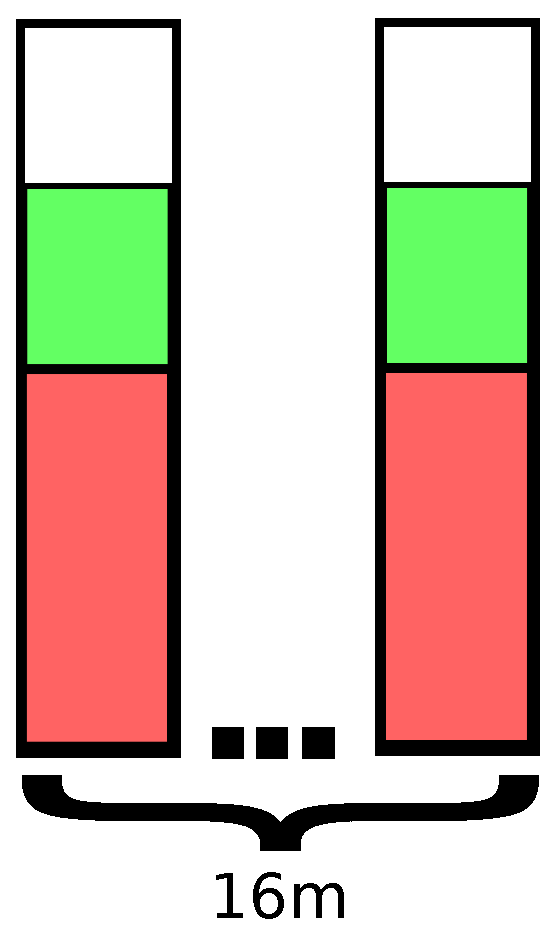
\includegraphics[scale=.3]{second}
\end{center}
\end{figure}
\end{multicols}

\begin{multicols}{2}
Nach Einfügen der $16m$ $\frac{1}{8}+\epsilon$ Objekte. 
\begin{figure}[H]
\begin{center}
	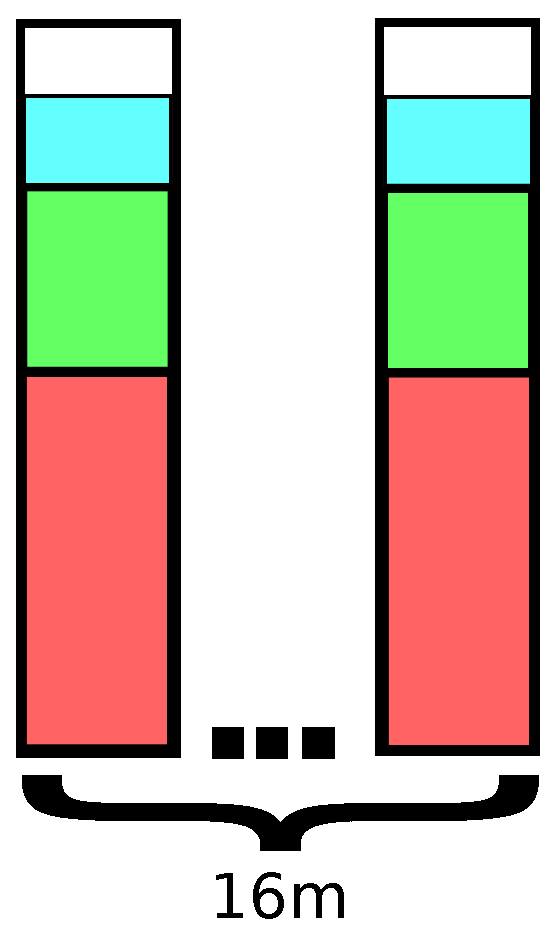
\includegraphics[scale=.3]{third}
\end{center}
\end{figure}
\columnbreak%
Nach Einfügen der $16m$ $\frac{1}{16}+\epsilon$ Objekte. 
\begin{figure}[H]
\begin{center}
	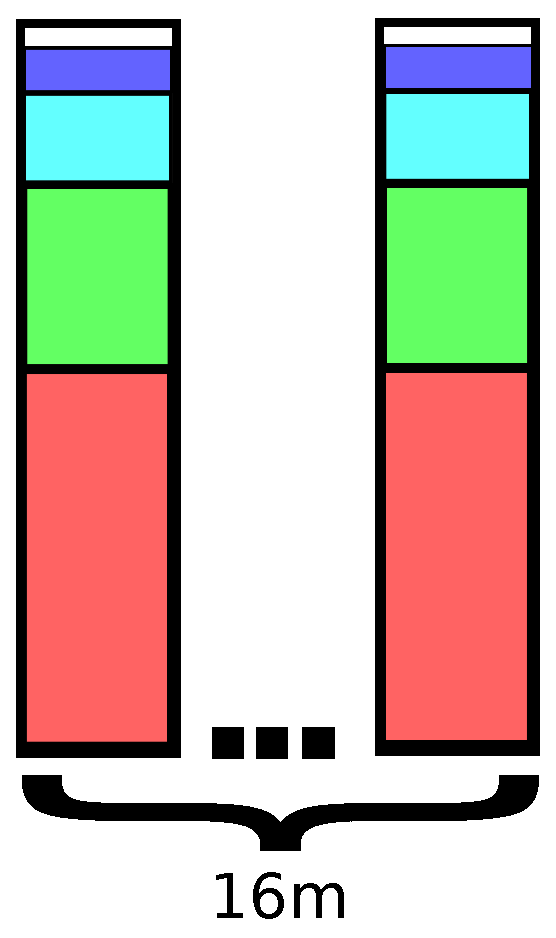
\includegraphics[scale=.3]{fourth}
\end{center}
\end{figure}
\end{multicols}

Keine zwei (gleich großen) Elemente einer $16m$ Objekte langen Teilsequenz stehen im selben Block.
\begin{align*}
(\frac{1}{2}+\epsilon)+(\frac{1}{2}+\epsilon) > 1\\
\implies (\frac{1}{2}+\epsilon)+2\cdot(\frac{1}{4}+\epsilon)\\ 
=(\frac{1}{2}+\epsilon)+(\frac{1}{4}+\epsilon)+2\cdot(\frac{1}{8}+\epsilon)\\
=(\frac{1}{2}+\epsilon)+(\frac{1}{4}+\epsilon)+(\frac{1}{8}+\epsilon)+2\cdot(\frac{1}{16}+\epsilon) > 1
\end{align*}
\newpage
Bei der angegebenen Belegung wird die Kapazität keines Blocks überschritten:\\
\begin{align*}
(\frac{1}{2}+\epsilon)+(\frac{1}{4}+\epsilon)+(\frac{1}{8}+\epsilon)+(\frac{1}{16}+\epsilon)\\
=(\frac{8}{16}+\epsilon)+(\frac{4}{16}+\epsilon)+(\frac{2}{16}+\epsilon)+(\frac{1}{16}+\epsilon)\\
=(\frac{15}{16}+4\epsilon)<1 
\end{align*}
da:\\
\begin{equation}
	\epsilon<\frac{1}{10^{6}} \implies 4\epsilon<\frac{1}{16}
\end{equation}
\begin{align*}
FFD(I)=OPT(I)=16m
\end{align*}

\clearpage%

{\bfseries Aufgabe 22}%

Geben Sie ein dynamisches Programm f{\"u}r die Berechnung von $\binom{n}{i}$ an.

\emph{Hinweis:} In der Vorlesung haben wir gezeigt, dass die Anzahl der Knoten
mit Tiefe $i$ in einem Binomialbaum $B_n$ genau $\binom{n}{i}$ entspricht.
Benutzen Sie die Argumente aus dem Beweis dieser Aussage.

Aus dem Beweis in der VO zu Binonmial Queues bzw. Binomialb{\"a}umen (
\emph{Es gibt genau $\binom{n}{i}$ Knoten mit Tiefe $i$ in $B_n$}) entnehmen wir
folgende Argumente:

\begin{equation}
\binom{n}{0} = 1 \text{ und } \binom{n}{n} = 1
\end{equation}

\begin{equation}
\binom{n}{i} = \binom{n - 1}{i} + \binom{n - 1}{i - 1}
\end{equation}

Diese beiden Gleichungen sind bereits eine rekursive Darstellung des
Binomialkoeffizienten $\binom{n}{i}$. F{\"u}r das dynamische Programm definieren 
wir nun analog dazu:

\begin{verbatim}
binom(n, 0) = 1
binom(n, n) = 1

binom(n, i) = binom(n - 1, i) + binom(n - 1, i - 1)
\end{verbatim}

Weiters ben{\"o}tigen wir eine $(n + 1)\times (i + 1)$-Matrix \texttt{coeff[][]},
in der wir bereits berechnete Ergebnisse speichern (Memorization-Array).

Mit diesen Bestandteilen l{\"a}sst sich das dynamische Programm formulieren. Das
dynamische Programm hat quadratische Laufzeit (in $n$) - im Gegensatz zu einer
naiven L{\"o}sung, welche exponentielle Laufzeit (in $n$) h{\"a}tte.

\begin{minipage}{.315\textwidth}
\begin{algorithm}[H]
    \small
%
    \SetKwProg{Fn}{Function}{}{}%
    \SetKwInOut{Input}{Input}%
    \SetKwInOut{Output}{Output}%
%
    \Input{$n$: \texttt{integer}, $i$: \texttt{integer}}%
    \Output{$\binom{n}{i}$: \texttt{integer}}%
    \Fn{binom($n$, $i$)}{%
        \For{$k \leftarrow 0$ \KwTo $n$}{
            \For{$l \leftarrow 0$ \KwTo $i$}{
                coeff[$k$][$l$] $\leftarrow$ $\infty$\;
            }
        }

        \For{$k \leftarrow 0$ \KwTo $n$}{
            coeff[$k$][$0$] $\leftarrow$ 1\;
            \For{$l \leftarrow 1$ \KwTo $i$}{
                coeff[$0$][$l$] $\leftarrow$ 0\;
            }
        }

        \Return lookupBinom($n$, $i$)\;
    }%
\end{algorithm}
\end{minipage}
\begin{minipage}{.635\textwidth}
\begin{algorithm}[H]
    \small
%
    \SetKwProg{Fn}{Function}{}{}%
    \SetKwInOut{Input}{Input}%
    \SetKwInOut{Output}{Output}%
    %
    \Input{$n$: \texttt{integer}, $i$: \texttt{integer}}%
    \Output{$\binom{n}{i}$: \texttt{integer}}%
    \Fn{lookupBinom($n$, $i$)}{%
        \If{coeff[$n$][$i$] = $\infty$}{
            coeff[$n$][$i$] $\leftarrow$ lookupBinom($n - 1$, $i$) + lookupBinom($n - 1$, $i - 1$)\;
        }

        \Return coeff[$n$][$i$]\;
    }%
\end{algorithm}
\end{minipage}

\end{document}
